% 第6章 本研究の詳細
\newpage
\renewcommand{\baselinestretch}{1.5}
\section{本研究の詳細}
\renewcommand{\baselinestretch}{1}

\par デザイナーやネットユーザーが検証するウェブページのURLおよびページのレイアウトタイプを入力すると該当ページの顕著性マップとページの構造を組み合わせることにより顕著度が高い領域を要素単位で分析して顕著領域マップを出力する手法を提案する。また、一般ユーザー向けに特に顕著度が高い領域を纏めて描写した集約図を出力する手法を提案する。本手法のモデルアーキテクチャを図\ref{fig_ourmodel}に示す。

\begin{figure}[H]
    \centering
    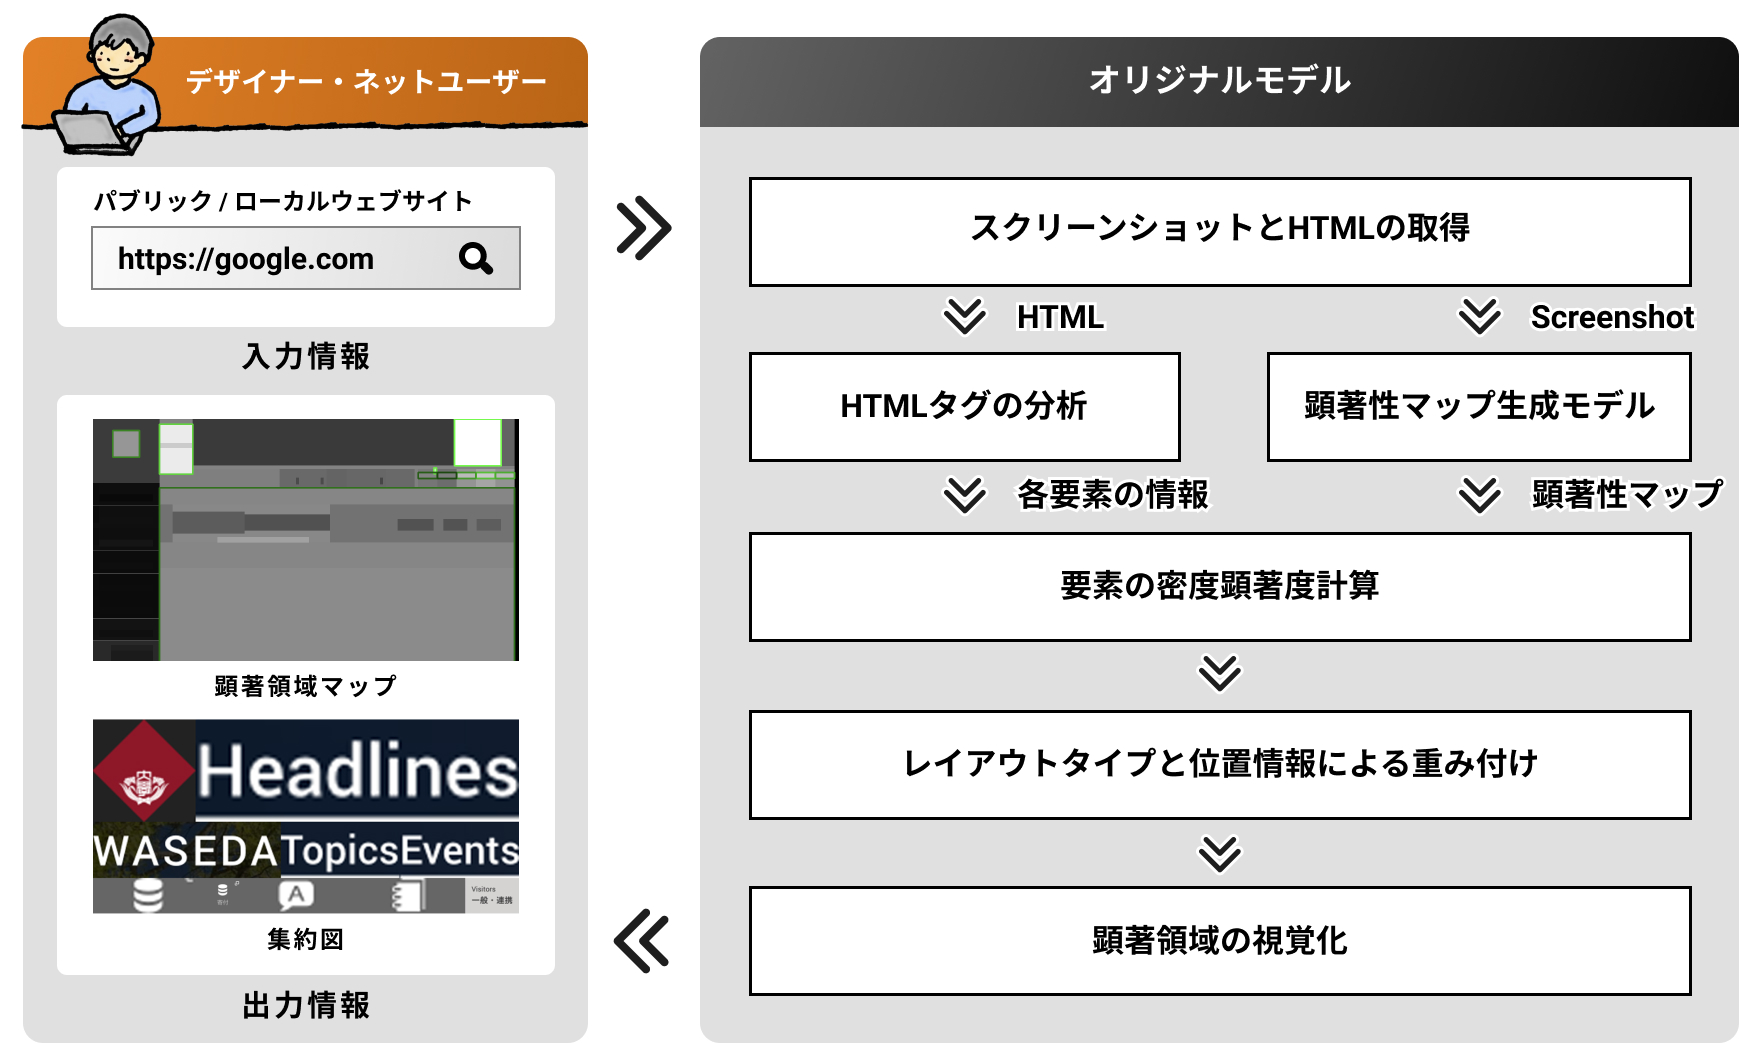
\includegraphics[width=9cm]{figures/model.jpg}
    \caption{モデルアーキテクチャ}
    \label{fig_ourmodel}
\end{figure}

\par 本手法の手順は大きく分けて以下の4つである。
\par(1) HTMLの取得と顕著性マップの生成
\par(2) HTMLの解析によるタグの分析と位置情報の取得
\par(3) レイアウトタイプを考慮した要素の顕著度計算
\par(4) 顕著領域の視覚化\\

\par なお、本研究ではサーバーサイドのプログラムを使用することで外部サーバーにアクセスしてウェブサイト上から必要な情報を取得するウェブスクレイピング技術としてウェブアプリケーションの自動テストツールであるSelenium WebDriver\cite{selenium}や取得したHTMLからタグや必要な情報を取得するPython用のライブラリであるBeautiful Soup\cite{beautifulsoup}を使用するが別のスクレイピング技術を使用しても実装は可能である。また、スクリーンショットを取得するウェブブラウザとしてFirefoxを使用するがChromeなど別のブラウザでも実装可能である。

\subsection{HTMLの取得と顕著性マップの生成}\label{subsec:system01}
\par 本システムではまず、入力されたURL情報を元にウェブスクレイピング技術を用いてスクリーンショットとHTMLを取得する。また、取得したスクリーンショットを用いて顕著性マップを生成する。デザイナーが開発段階で簡単に使用可能な様に入力するURLは、ネットワーク上に存在するウェブページだけでなくローカル環境のURLにも対応させている。HTMLの取得と顕著性マップの生成の流れを図\ref{fig_system01}に示す。

\begin{figure}[H]
    \centering
    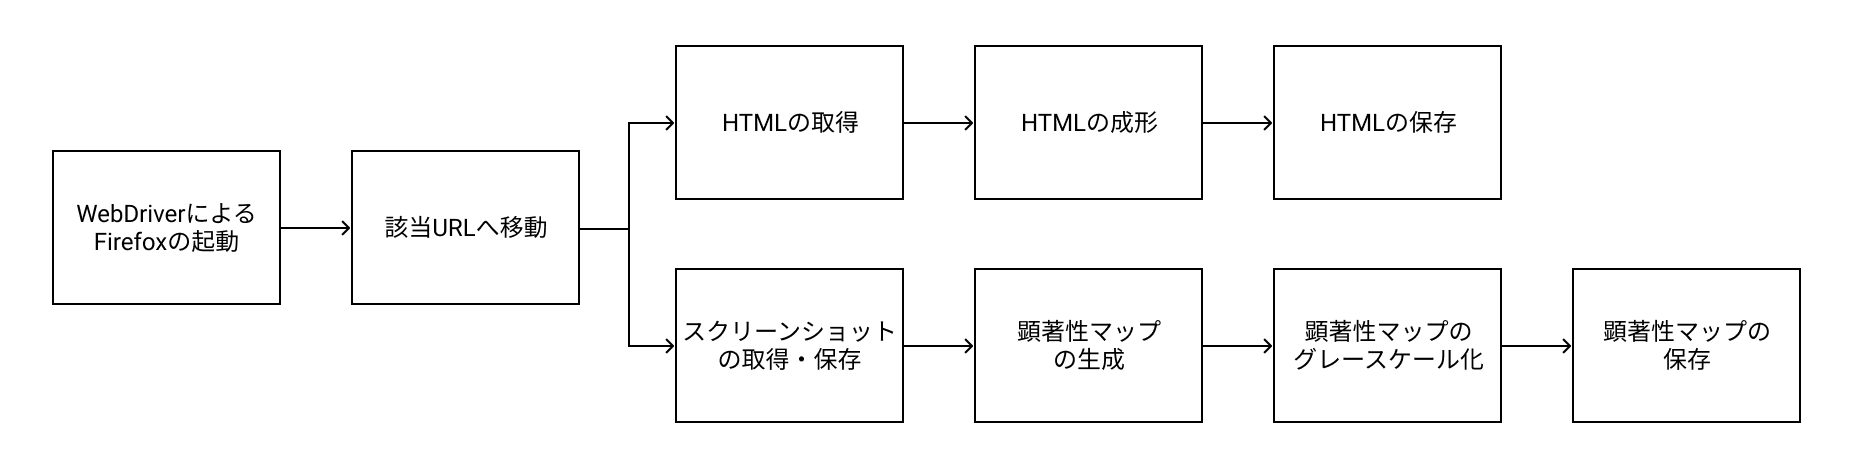
\includegraphics[width=12cm]{figures/06_process01.jpg}
    \caption{HTMLの取得と顕著性マップの生成の流れ}
    \label{fig_system01}
\end{figure}

\par まず始めに、Selenium WebDriverを用いてFirefoxを起動し、ブラウザのウィンドウサイズを一般的なパソコンで閲覧する条件に近い横1280px縦900pxに設定する。次に入力されたURLにアクセスを行い、ウェブページの読み込みが完了したらHTMLの取得を行う。取得したHTMLはインデントなどが乱れた状態である為、Selenium WebDriverと同じくウェブスクレイピング技術のライブラリであるBeautiful Soup\cite{beautifulsoup}を使用して扱いやすい状態に整形を行った後に保存する。

\par 次にウェブページのスクリーンショットを取得する。取得するスクリーンショットは、重要度が高いコンテンツはウェブページの最上部に存在する可能性が高いという考えから、ウェブページにアクセスした時点で閲覧可能な最上部の横1280px縦900pxとした。さらに、取得したスクリーンショットから顕著性マップを生成する。顕著性マップの生成には人間の目の視覚認識と同様に色・輝度・方向のそれぞれの視覚特徴を抽出した後に重み付けして足し合わせることにより顕著性マップを生成する最もベーシックなモデルのItti-Kochらの顕著性マップ生成モデルをベースに使用した。顕著性マップ生成モデルには深層学習を使用した精度の高いモデルまで幅広く存在しているが、特にバイアスを考慮しておらず扱いやすいモデルを使用することにした。
\par ここで顕著性マップ生成モデルにより出力される顕著性マップはRGBの3色チャンネルで出力されるが、計算処理を行いやすいように単色チャンネルで表されるグレースケール画像に変換して保存する。図\ref{fig_06_example_saliencymap}に早稲田大学ウェブサイトトップページ(2021年1月時点)\cite{waseda_top}のスクリーンショットを入力した時に生成される取得されるグレースケール顕著性マップの例を示す。

\begin{figure}[H]
  \centering
  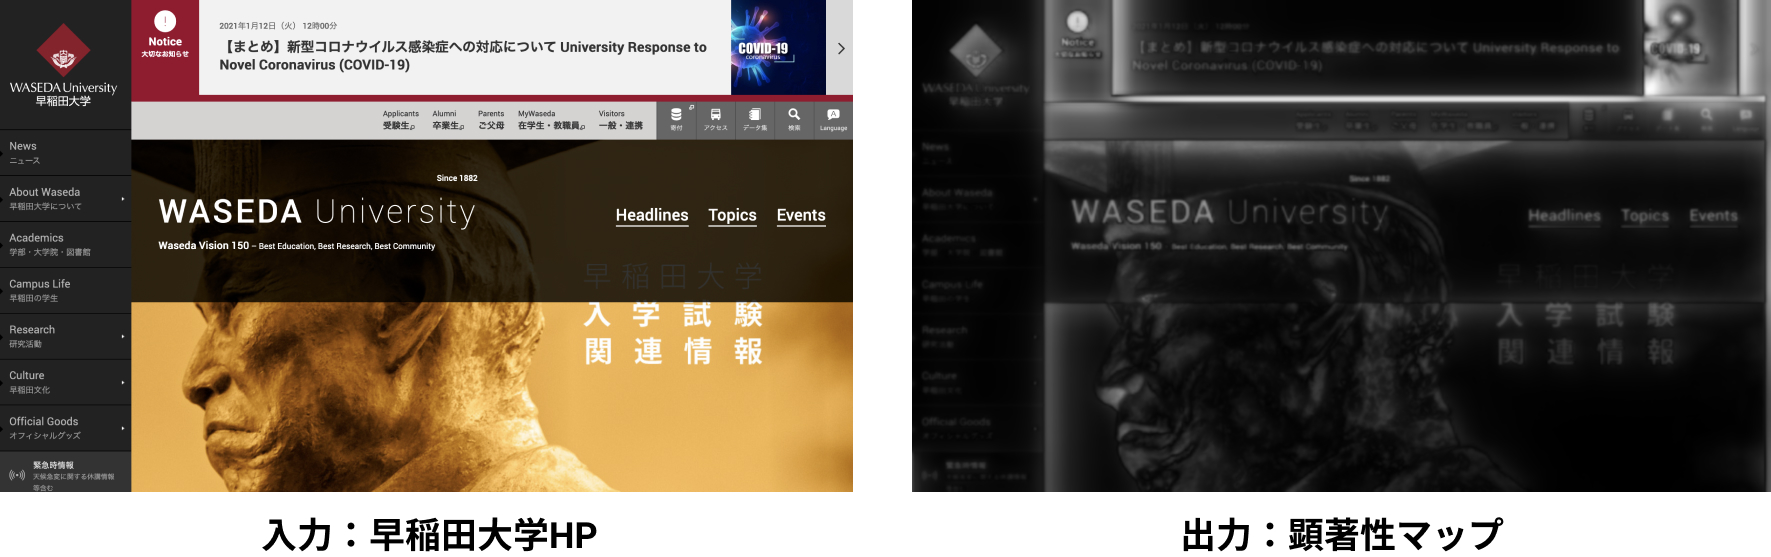
\includegraphics[width=12cm]{figures/06_ex-saliencymap}
  \caption{出力されるウェブページの顕著性マップの例}
  \label{fig_06_example_saliencymap}
\end{figure}


\subsection{HTMLの解析によるタグの分析と位置情報の取得}\label{subsec:system02}
\par ここでは第\ref{subsec:system01}節で取得したHTMLの解析を行いウェブページ上の要素の位置情報とそのサイズを取得する。HTMLの解析によるタグの分析と位置の取得の流れを図\ref{fig_system02}に示す。

\begin{figure}[H]
    \centering
    
\includegraphics[width=12cm]{figures/06_process02.jpg}
    \caption{HTMLの解析によるタグの分析と位置の取得の流れ}
    \label{fig_system02}
\end{figure}

\par まず始めに第\ref{subsec:system01}節で取得したHTMLの分析を行い、Selenium WebDriverで表\ref{table:gettaglist}に示す7個のタグ要素のidまたはclass名と左上の頂点の座標と縦と横のサイズを取得してそれらの情報をデータベースに記録する。各要素の座標の取得方法については、ウェブブラウザの表示領域の左上を基準点(0,0)として基準点からの距離を要素の座標とした。また、時間短縮とエラーを防ぐために取得したスクリーンショット領域内に表示されている要素のみを取得する。早稲田大学ウェブサイトトップページ(2021年1月時点)\cite{waseda_top}および、Yahoo! JAPANトップページ(2021年1月時点)\cite{yahoo}のウェブページの要素情報を取得して、直線で各要素を囲んだ例を図\ref{fig_06_ex-lineview}に示す。表示領域の指定要素のサイズと位置を取得している事が確認できる。

\begin{table}[h]
    \caption{位置情報とサイズを取得するタグの一覧}
    \label{table:gettaglist}
    \centering
     \begin{tabular}{clll}
      \hline
      要素名 & タグ & 意味 \\
      \hline \hline
      ブロック要素 & \textless div\textgreater & ブロック要素を表す \\
      見出し1 & \textless h1\textgreater & 文書中の見出しを示す為の要素で最も重要 \\
      見出し2 & \textless h2\textgreater & 文書中の見出しを示す為の要素で2番目に重要 \\
      見出し3 & \textless h3\textgreater & 文書中の見出しを示す為の要素で3番目に重要 \\
      リンク & \textless a\textgreater & リンクを示す \\
      インライン要素 & \textless span\textgreater & インライン要素を示し、重要な要素が多い \\
      段落 & \textless p\textgreater & テキスト要素を表す \\
      入力欄 & \textless input\textgreater & フォームなどの入力要素を表す \\
      イメージ & \textless img\textgreater & 画像要素を表す \\
      \hline
    \end{tabular}
\end{table}

\begin{figure}[H]
  \centering
  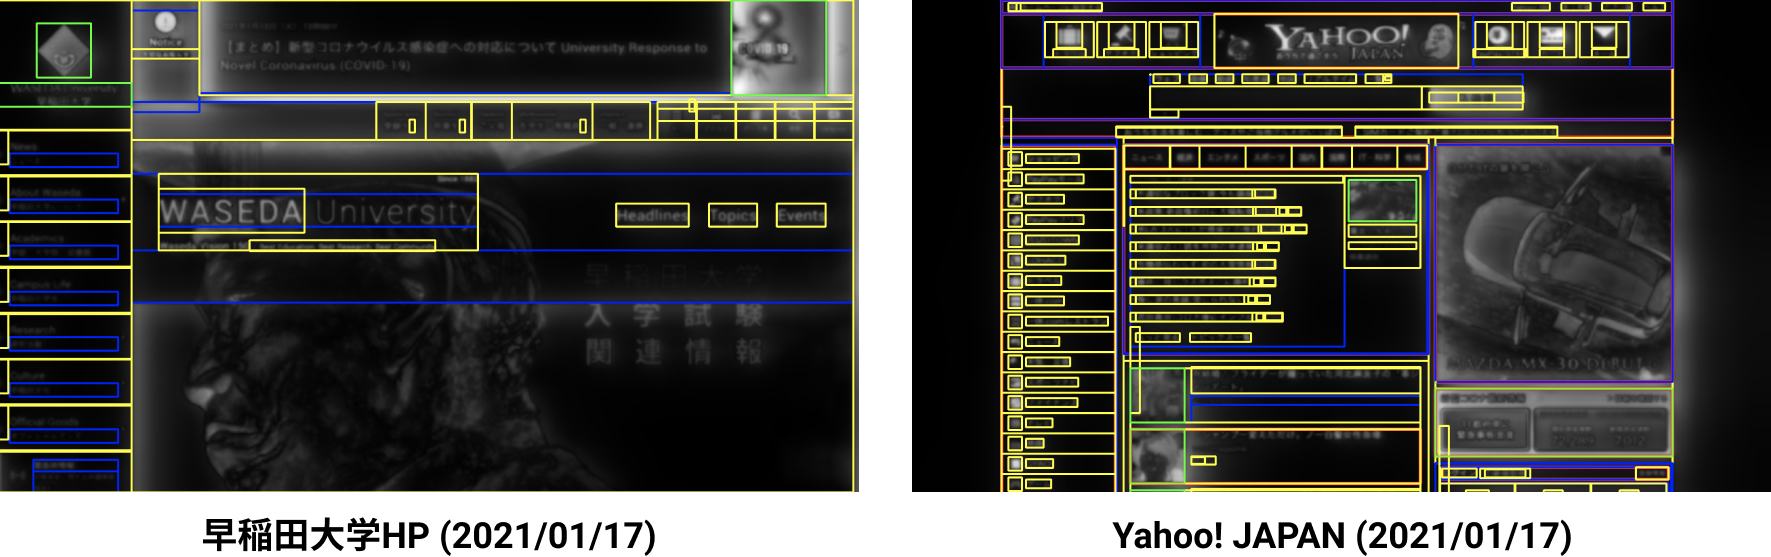
\includegraphics[width=12cm]{figures/06_ex-lineview.jpg}
  \caption{ウェブページの要素の取得の様子}
  \label{fig_06_ex-lineview}
\end{figure}

\subsection{レイアウトタイプを考慮した要素の顕著度計算}\label{subsec:system03}
\par ここでは第\ref{subsec:system01}節で生成した顕著性マップと第\ref{subsec:system02}節で取得した各要素の位置情報とサイズを組み合わせて各要素の顕著度を計算する。レイアウトタイプを考慮した要素内顕著度の計算の流れを図\ref{fig_system03}に示す。

\begin{figure}[H]
    \centering
    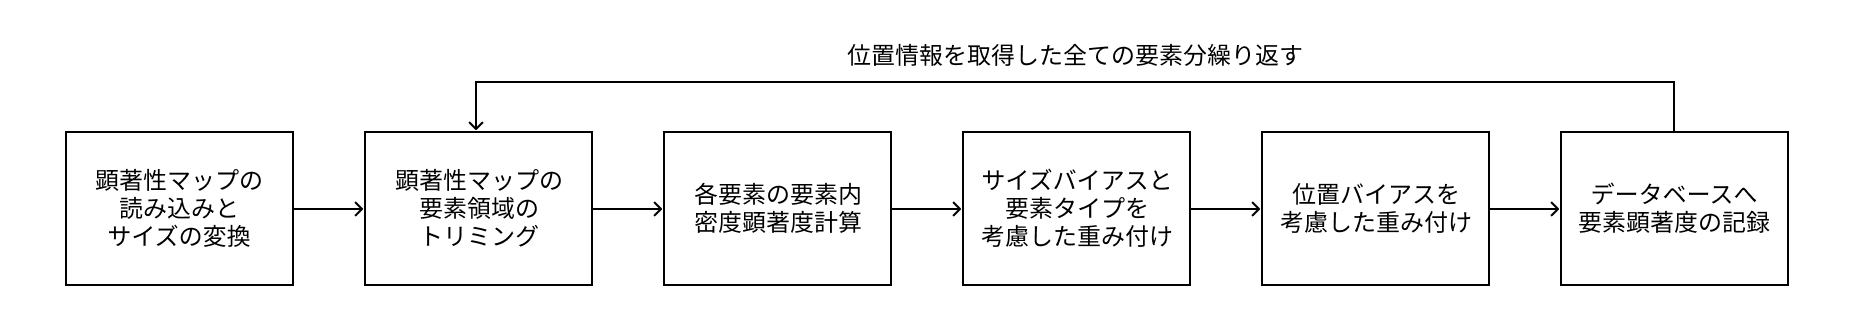
\includegraphics[width=12cm]{figures/06_process03.jpg}
    \caption{顕著度の計算の流れ}
    \label{fig_system03}
\end{figure}

\par まず始めに第\ref{subsec:system01}節で作成した顕著性マップを読み込む。使用端末により異なるが最近のパソコンは画面の高画質化が進み、AppleのRetinaディスプレイなどの高精細ディスプレイでは複数のピクセルで1つのドットを表しており倍近い解像度でスクリーンショットが保存されている。その為、単純に顕著性マップを読み込み要素の位置情報と照らし合わせるとズレが生じる。この問題を解決する為に読み込んだ顕著性マップを圧縮して実際にウェブブラウザ上で取得した位置情報と同じサイズに合わせる必要がある。

\par 次に第\ref{subsec:system02}節で取得した各要素ごとの顕著度を計算するために顕著性マップの該当要素の領域をトリミングする。また、トリミングした領域のピクセルレベルでの顕著度の積分を要素面積の平均顕著度で割る事で要素の密度顕著度を計算する。具体的な計算方法をアルゴリズム\ref{alg:element_saliency}に示す。従来は要素内部のピクセルレベルの顕著度の平均を顕著度としていたが、要素のピクセルレベルでの密度顕著度を計算したことで、小さな要素から大きい要素までバランスよく顕著度を評価する事が可能である。

\par しかしながらアイコンなどの極端に小さい要素の顕著度が過剰に高く評価されてしまうなどの問題が生じた。またウェブページの左上から中央にかけての領域に視線が集まりやすいf-biasなどのウェブページ固有の現象なども存在する。それらの問題を解決するために、本システムでは要素のサイズと位置情報によるレイアウトを考慮した顕著度の重み付けを行う事でより正確に顕著度を判定出来るように工夫した。

\begin{algorithm}[H]
  \small
  \caption{要素の顕著度計算手法}
  \label{alg:element_saliency}
  \begin{algorithmic}
  \Function{get\_element\_salient\_level}{start\_x, start\_y, end\_x, end\_y}
  \If{(end\_x - start\_x) $>$ 0 and (end\_y - start\_y) $>$ 0}
    \State cliped = Element.canvas.cv2[start\_y:end\_y, start\_x:end\_x] //要素をトリミング
    \State element\_occupancy = $\frac{(end\_x - start\_x) \times (end\_y - start\_y)}{width * height}$ //要素の占有率を計算
    \State salient\_level = $\frac{get\_element\_total\_saliency(cliped)}{get\_total\_saliency() \times element\_occupancy}$ //要素の顕著度を計算
    \State \Return salient\_level
  \Else
    \State \Return 0
  \EndIf
  \EndFunction
  \State
  \Function{get\_total\_saliency}{}
    \State clipped = Element.canvas.cv2[0:height, 0:width] //ウェブページ全体
    \State total\_saliency\_per\_row = np.sum(clipped, axis=0) //行の色の合計を取得
    \State total\_saliency = np.sum(total\_saliency\_per\_row, axis=0) //列の色の合計を取得
    \State \Return np.uint8(total\_saliency)
  \EndFunction
  \State
  \Function{get\_element\_total\_saliency}{clipped}
    \State total\_saliency\_per\_row = np.sum(clipped, axis=0) //行の色の合計を取得
    \State total\_saliency = np.sum(total\_saliency\_per\_row, axis=0) //列の色の合計を取得
    \State \Return np.uint8(total\_saliency)
  \EndFunction
  \end{algorithmic}
\end{algorithm}

\subsubsection{要素のサイズと要素タイプによる重み付け}\label{subsec:system03-1}
\par 先ほど述べた通り、アイコンなどの極端に小さい要素の顕著度が極端に高く計算される傾向があることが判明した為、要素の大きさによる重み付けを行うことで顕著度の偏りをなくす。ウェブページに存在するアイコンには様々なサイズのものが存在する。また画像要素だけでなく、CSSで描写されたアイコンやdiv要素にbackgroundプロパティで指定されたものなど要素のタイプも様々である。そこで本システムでは一般的にアイコンと呼ばれるサイズ以下の要素の重みを変更して適切な顕著度を計算する事にした。

\par 我々が日常でよく閲覧するアイコンとしてWindowsやMacやIOSなどのOS標準のアイコンが存在する。MicrosoftによるとWindowsではダイアログボックスやエラーページなどに32px$\times$32pxのアイコンが標準サイズとして使用されている\cite{windowsicon}。また、iPhoneなどのIOSやMacには64px$\times$64pxのアイコンが標準サイズとして使用されている\cite{appleicon}。日常でよく使用するアイコンのサイズのほとんどは32px$\times$32pxおよび64px$\times$64pxであることから人はこれらのサイズの要素をアイコンと認識する傾向が高い。以上のことから本システムでは64px$\times$64px以下のサイズの要素をアイコン要素とみなして顕著度を低く重み付けするようにアルゴリズムを\ref{alg:weight-size}のように設定した。なお、重み付けの値については本来であれば深層学習等を用いて適切な重み付けを学習するのが良いが、極端に小さな要素の顕著度を適切に判断できるように様々な値で繰り返し実験を行い最も実際の顕著度に近くなった値を設定した。

\begin{algorithm}[H]
  \small
  \caption{サイズによる重み付け}
  \label{alg:weight-size}
  \begin{algorithmic}
  \Function{apply\_size\_bias}{salient\_level, start\_x, start\_y, end\_x, end\_y}
  \State element\_area =  (end\_x - start\_x) $\times$ (end\_y - start\_y) //要素の面積を計算
  \If{element\_area $>$ 64 $\times$ 64 }
    \State salient\_level = salient\_level
  \Else
    \State salient\_level = salient\_level $\times$ 0.5
  \EndIf
  \State \Return salient\_level
  \EndFunction
  \end{algorithmic}
\end{algorithm}

\begin{figure}[H]
  \centering
  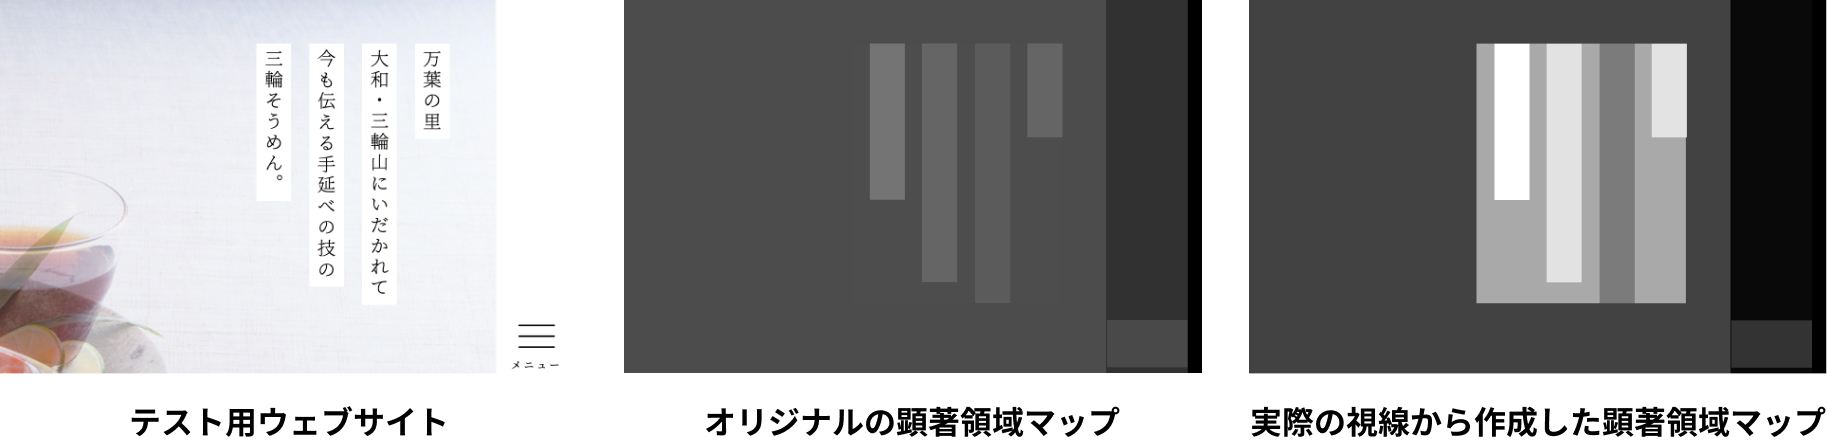
\includegraphics[width=12cm]{figures/06_textbias.jpg}
  \caption{テキスト箇所の顕著性評価比較}
  \label{fig_textbias}
\end{figure}

\par ウェブページには自然画像とは異なり様々なウェブページ固有の要素が存在する。その中の一つであるテキスト要素は自然画像にはほとんど存在せずあまり顕著度が高く評価されないがウェブページには多く存在する。図\ref{fig_textbias}にウェブページのテキスト表示箇所のオリジナルモデルの顕著領域マップと実際の視線データから作成した顕著領域マップの比較を示す。図から分かる通り人はテキスト要素に注目する傾向が高いが、Itti-Kochらのモデルなどの自然画像向け顕著性マップ生成モデルはテキストの顕著度をあまり高く評価しない。テキスト要素の顕著度を正しく評価するために該当要素の顕著度を高くするように重み付けを行った。


\subsubsection{要素の位置とレイアウトによる重み付け}\label{subsec:system03-2}
\par 関連研究でも触れたが有名なものとしてウェブページには自然画像と異なり、左上から中央付近の領域に存在する要素が注目されやすい傾向があるf-biasというバイアスが存在する。図\ref{fig_gazetime}に第\ref{subsec:gazedataset}節で作成した被験者がデータ分析用のウェブページを10秒間閲覧した際の実際の視線座標データを3秒間ずつヒートマップに表したものを示す。一番右の10秒間全ての視線座標データを合成したヒートマップを見ると左上から中央付近の要素に注目が集まりやすい傾向があるのは明らかである。また時間帯ごとの視線座標の推移を確認すると、最初の3秒間は左上から中央の領域が顕著に注目されている事が確認できる。また、3000ms-6000msや6000-9000msのヒートマップを見ると時間が経過するにつれて被験者の視線は左上から中央付近にかけて移動してより幅広い範囲に広がっている事が確認できる。このように昔からのベーシックデザインだけでなく近年の主流になっているモダンデザインにおいてもf-biasが適応可能である。また、時間の経過につれて注目される領域が大きく変化する事が明らかになった。

\begin{figure}[H]
  \centering
  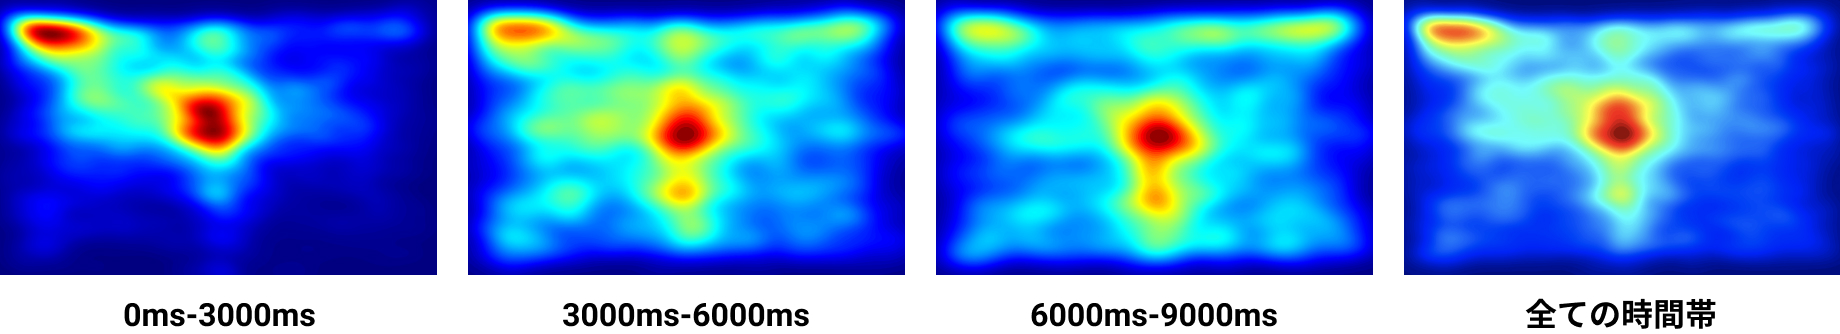
\includegraphics[width=12cm]{figures/06_gazetime.jpg}
  \caption{各時間帯ごとの平均顕著性ヒートマップ}
  \label{fig_gazetime}
\end{figure}

\par このようなウェブページ固有の視線のバイアスを反映させる為に本システムでは要素の位置情報ならびにウェブページのレイアウトタイプによる重み付けを行う。従来の研究では左上の領域に大きな重みをつけるtop-left biasを横軸方向と縦軸方向にそれぞれ重みを付ける事で擬似的に表現していた。また、中心領域に大きな重みをつけるcenter biasにおいては中心部と最外部でどれだけ重みの差をつけるかを表す重みを設定する事で表現していた。しかしながらこれらの手法では全てのレイアウトにおいて同じ擬似的なバイアスを適応させることになり顕著度評価の正確性はあまり高くない。そこで本研究ではレイアウトタイプによる重み付けを行い、各レイアウトごとの視線データの推移の傾向を分析して結果を適応する。図\ref{fig_layout_result}に各レイアウトに所属するウェブページの中央点とその移動の軌跡を示す。図\ref{fig_layout_result}の×マークはそれぞれのレイアウトに所属する各ウェブページの2秒間の視線座標の平均座標である。また大きく外れているものを除いて各ウェブページの平均座標の全てが含まれるように作成された楕円の中心座標を中央点と呼び、ウェブページ上の要素の中心がこの楕円の中に含まれる場合は閲覧される可能性が高いことを示す。なお、10秒間の閲覧を2秒ごとに区切ることで各時間帯ごとの視線の推移を確認する事が可能である。シングルカラムパターンや2カラムパターンなどのカラムレイアウトは左上の領域から中央の領域にかけて注目されている一方で、ブロークングリッドパターンやフルスクリーンパターンなどのモダンデザインレイアウトは時間の経過による視線の動きはあまり大きくなく、中央付近の要素が注目されやすい。これらの特徴を利用して位置情報とレイアウトによる重み付けを行う。本システムの重み付けの手法をアルゴリズム\ref{alg:weight-position}に示す。

\par まず初めに調査対象のウェブページのレイアウトの顕著領域情報を表\ref{table:layoutresult}より取得する。次にウェブページの各要素の中心座標が取得した顕著領域の中に入っているかどうかを$judge\_inside\_ellipse$関数で調査する。調査方法については、2秒ごとの合計5つの時間帯の楕円顕著領域のいずれかに要素の中心座標が存在するかどうかを確認して存在する場合は注目される可能性が高いことを示す。注目される可能性が高い要素については反復実験から決定した位置バイアスの重み$weight\_position$を乗算することで要素の顕著度の重み付けを行う。

\par 図\ref{fig_positionbias}にテスト用ウェブページを入力した時の各レイアウトの要素の位置情報による重み付けのシミュレーション結果を示す。テスト用ウェブページは左上の画像のように白色の背景上に黒色の正方形を等間隔で並べたものを使用した。最上部中央の画像のように重み付け前の顕著性マップでは全ての正方形が同じ明度で表わされているが、位置情報による重み付け後の顕著性マップでは第\ref{subsec:gazedataset}節で分析した結果を用いて各レイアウトの左上から中央付近の顕著領域のの正方形の明度が高く表わされている事が確認できる。なお、認識しやすいように重み付け後の顕著領域マップには顕著度のランキングを緑色の枠線の色で表しており、明緑色になるほど顕著度が高く評価されていることを示す。

\par 最後に、要素毎にサイズと要素タイプならびに位置情報による重み付け処理を行なった結果の顕著度を最終的な出力に使用する為にデータベースに保存する。

\begin{algorithm}[H]
  \small
    \caption{位置情報とレイアウトパターンによる重み付け}
    \label{alg:weight-position}
    \begin{algorithmic}
    \Function{apply\_position\_bias}{salient\_level, start\_x, start\_y, end\_x, end\_y, type}
    \State weight\_position $\leftarrow$ 位置バイアスの重み
    \State bias\_info\_list $\leftarrow$ レイアウトの中心座標のリスト
    \State center\_x = (start\_x + end\_x) / 2 //中心x座標
    \State center\_y = (start\_y + end\_y) / 2 //中心y座標
    \For{\texttt{<bias\_info\_list>}}
      \If{ judge\_inside\_ellipse(center\_x, center\_y, bias\_info) }
        \State \Return salient\_level $\times$ weight\_position
      \Else
        \State \Return salient\_level
      \EndIf
    \EndFor
    \EndFunction
    \State
    \Function{judge\_inside\_ellipse}{center\_x, center\_y, bias\_info}
      \State \Return 中心座標が楕円の中に存在するかどうかを返す
    \EndFunction
    \end{algorithmic}
\end{algorithm}

\begin{figure}[H]
    \centering
    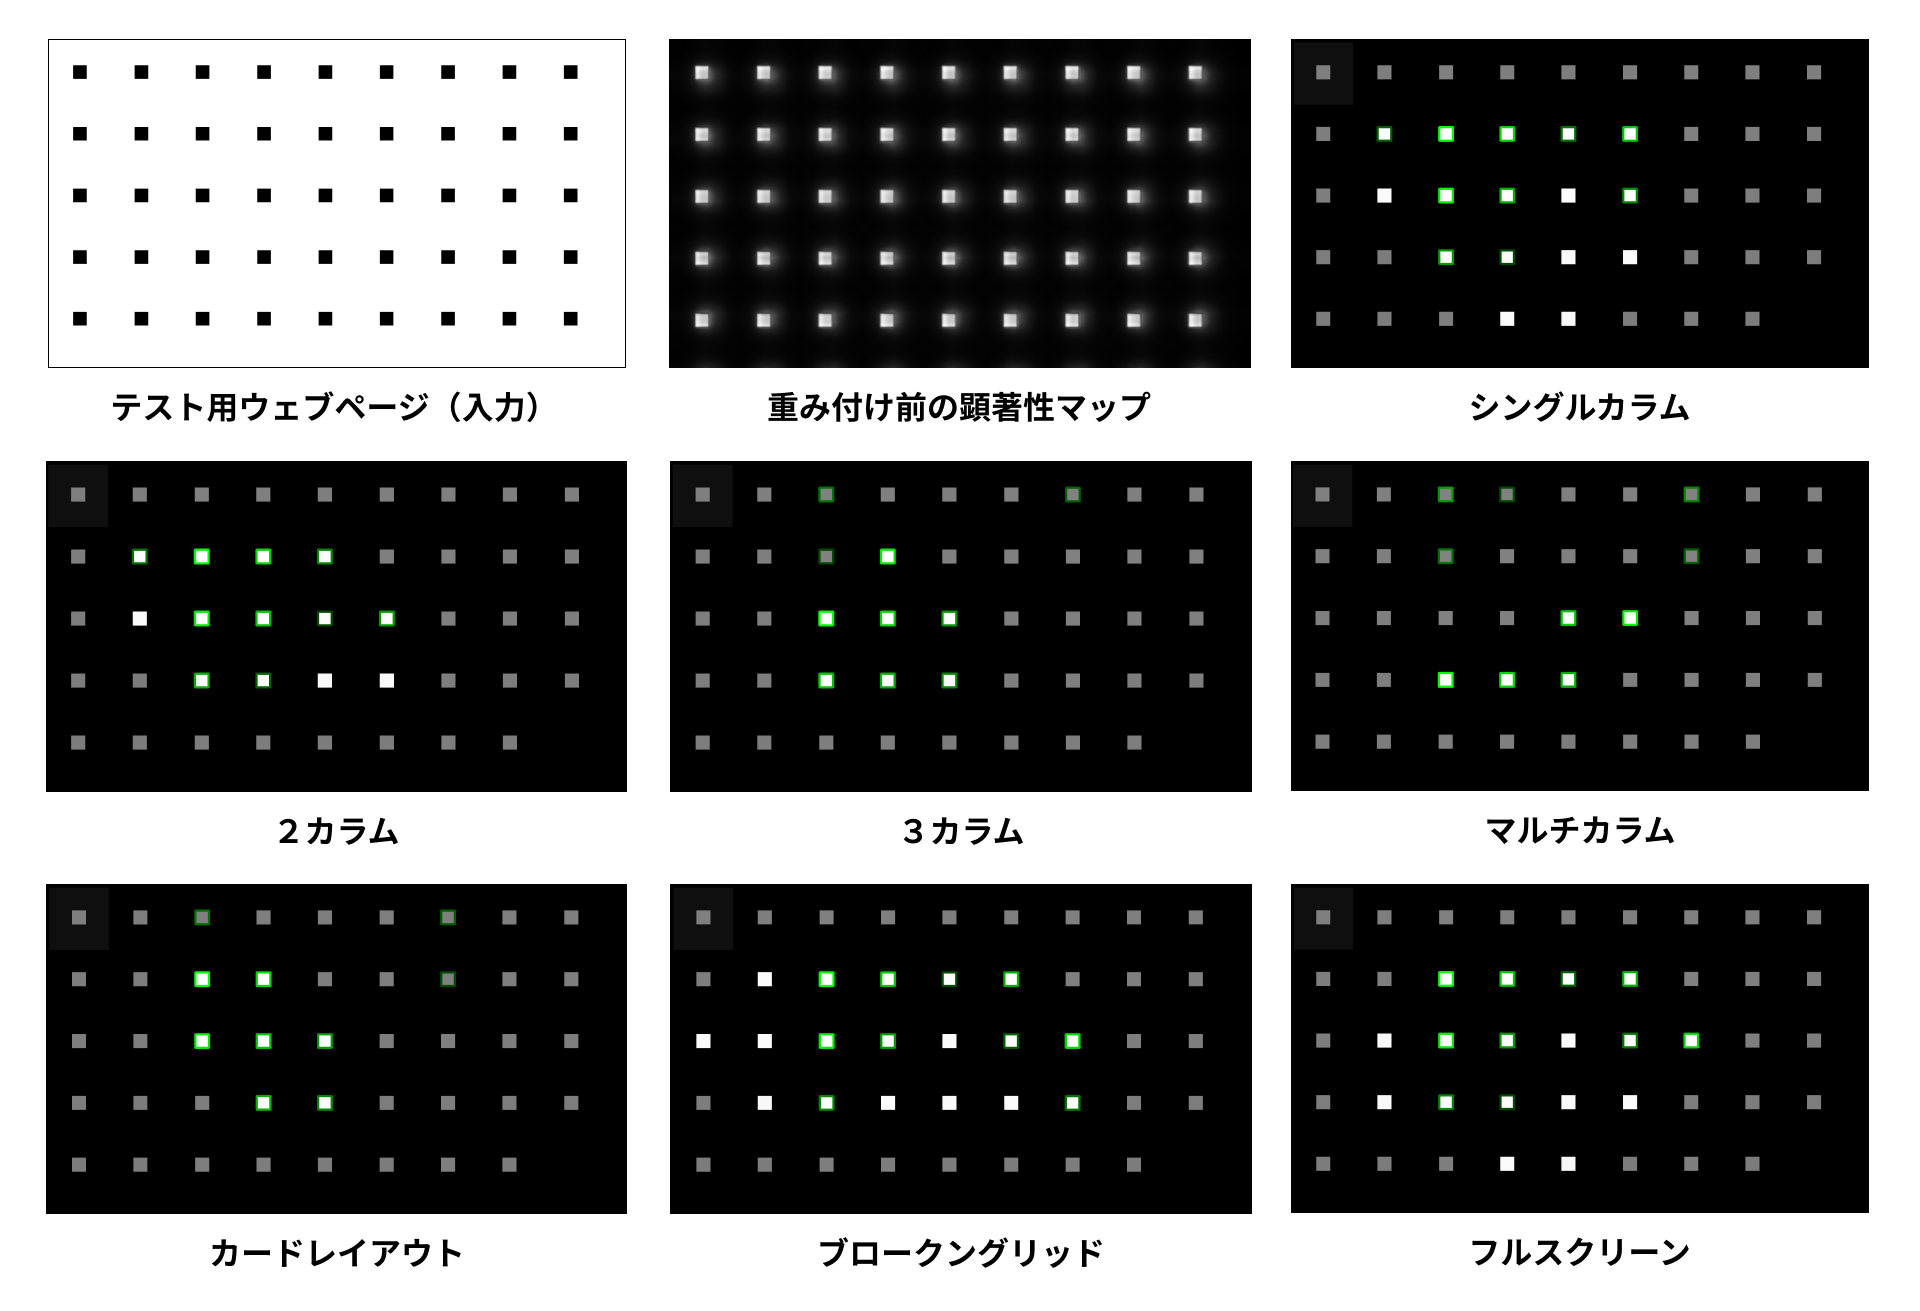
\includegraphics[width=12cm]{figures/06_positionbias.jpg}
    \caption{位置情報による重み付けのシミュレーション}
    \label{fig_positionbias}
\end{figure}


\subsection{顕著領域の視覚化}\label{subsec:system04}
\par ここでは第\ref{subsec:system03}節で計算した要素ごとの顕著度を元に顕著領域の視覚化を行う。本システムでは、顕著度が高い重要領域を要素単位で塗りつぶした顕著領域マップと特に顕著度が高い要素を一つにまとめた集約図の2つの出力を行う。顕著領域の視覚化の流れを図\ref{fig_system04}に示す。

\begin{figure}[H]
    \centering
    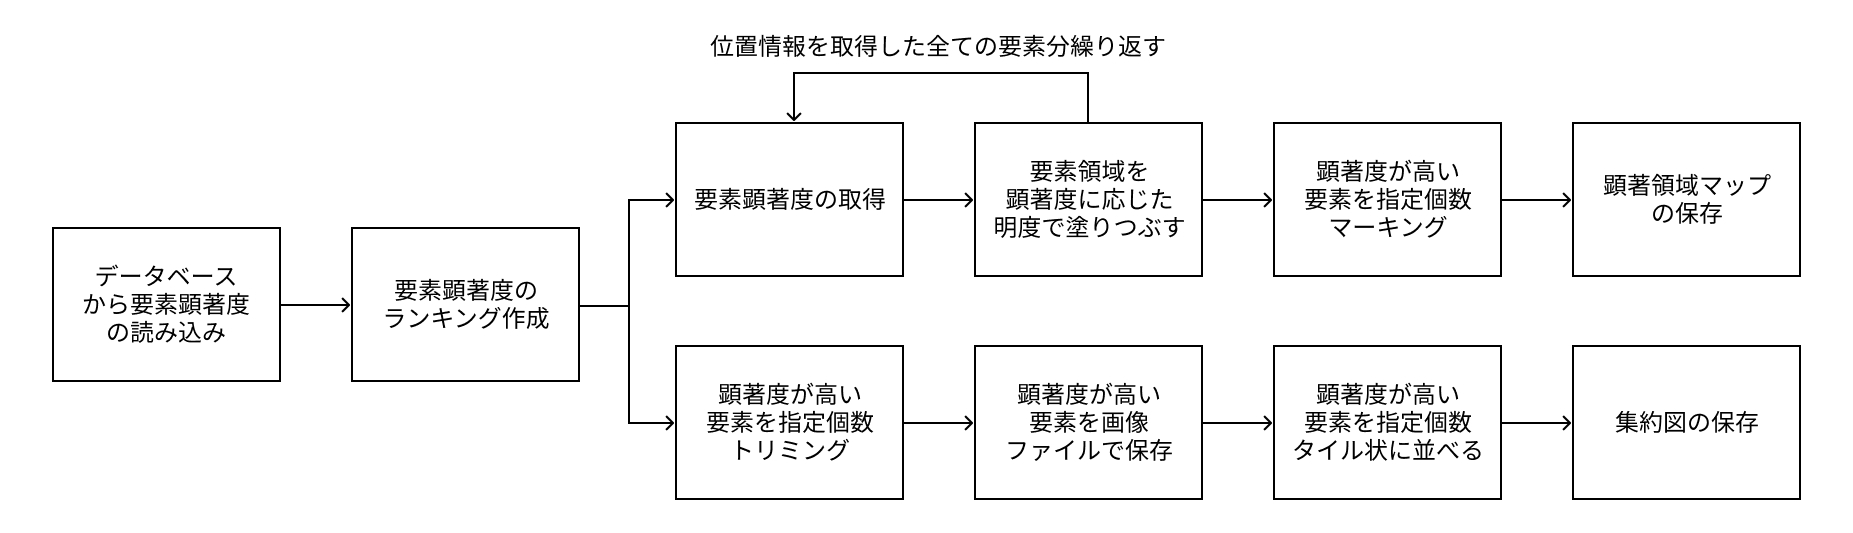
\includegraphics[width=12cm]{figures/06_process04.jpg}
    \caption{顕著領域の視覚化の流れ}
    \label{fig_system04}
\end{figure}

\subsubsection{顕著度ランキングの生成}\label{subsec:system04-1}
\par 顕著領域マップと集約図の生成にあたり、第\ref{subsec:system03}節で計算した顕著度のランキングを作成する。顕著度ランキングの計算アルゴリズムをアルゴリズム\ref{alg:lanking}に示す。まず始めに、第\ref{subsec:system03}節でデータベースに保存した顕著度を顕著度が高い順にソートする。本来であれば、顕著度が高い順にランキングを付ければ良いが、図\ref{fig_system4-rank}に示すように同一要素を内包している他の要素も顕著度が高く評価されてしまう問題が生じる。同じ要素が顕著度ランキングに何度も出現する事は問題である為、一度顕著度が高いと評価した要素を内包する外部の要素をNGリストに格納して顕著度ランキングに入らないように評価する。また、ウェブページの要素の中には装飾等の為に極端に細長い要素など顕著度ランキングに不必要なノイズが存在する。これらの要素を取り除く為にフィルターをかけて極端な形状の要素を取り除いた。

\newpage
\begin{algorithm}[H]
  \small
  \caption{顕著度ランキング}
  \label{alg:lanking}
  \begin{algorithmic}

  \State stag\_list $ \leftarrow $ CSVの読み組み
  \State tag\_list\_num $ \leftarrow $ CSVの行数
  \State salient\_level = [] // 顕著度を格納するリスト
  \State ng\_list = [] // NGリスト
  \State high\_element\_list = [] // 顕著度ランキングを格納するリスト
  \For{$i$ in $range(tag\_list\_num)$}
    \State salient\_level.append(tag\_listのi行目の要素の顕著度)
  \EndFor    
  \State salient\_level\_sort $ \leftarrow $ salient\_levelをソート
  \State salient\_num $ \leftarrow $ 10 //顕著度ランキングを生成する個数
  \State temporal\_num $ \leftarrow $ 1
  \State salient\_num\_first $ \leftarrow $ salient\_num

  \While{while salient\_num $>$ 0}
    \State most\_salient $ \leftarrow $ salient\_level\_sort[tag\_list\_num - temporal\_num]
    \If{(most\_salient in ng\_list) == False}
    \State start\_x, start\_y, end\_x, end\_y $\leftarrow$ CSVのmost\_salient行目から取得
    \State size $\leftarrow$ CSVからmost\_salient行目の要素のwidth $*$ heightを取得
    \If{(end\_x $-$ start\_x)/(end\_y $-$ start\_y) $<$ 10}
    \State high\_element\_list.append(most\_salient)
    \State salient\_num $\leftarrow$ salient\_num - 1
    \For{$i=1$ in $range(tag\_list\_num)$}
    \If{(most\_salient in ng\_list) == False}
    \State r\_start\_x, r\_start\_y, r\_end\_x, r\_end\_y $\leftarrow$ i行目から取得
    \State r\_size $\leftarrow$ CSVからi行目の要素のwidth*heightを取得
    \If{i行目要素とmost\_salient行目要素が内包関係}
    \If{r\_size $-$ size $<$ 200 $or$ size $-$ r\_size $<$ 200}
    \State ng\_list.append(i) //NGリストにi行目要素を格納
    \EndIf
    \EndIf
    \EndIf
    \EndFor 
    \EndIf
    \Else
    \State temporal\_num $\leftarrow$ temporal\_num $+$ 1
    \EndIf
  \EndWhile
  \end{algorithmic}
\end{algorithm}

\begin{figure}[H]
    \centering
    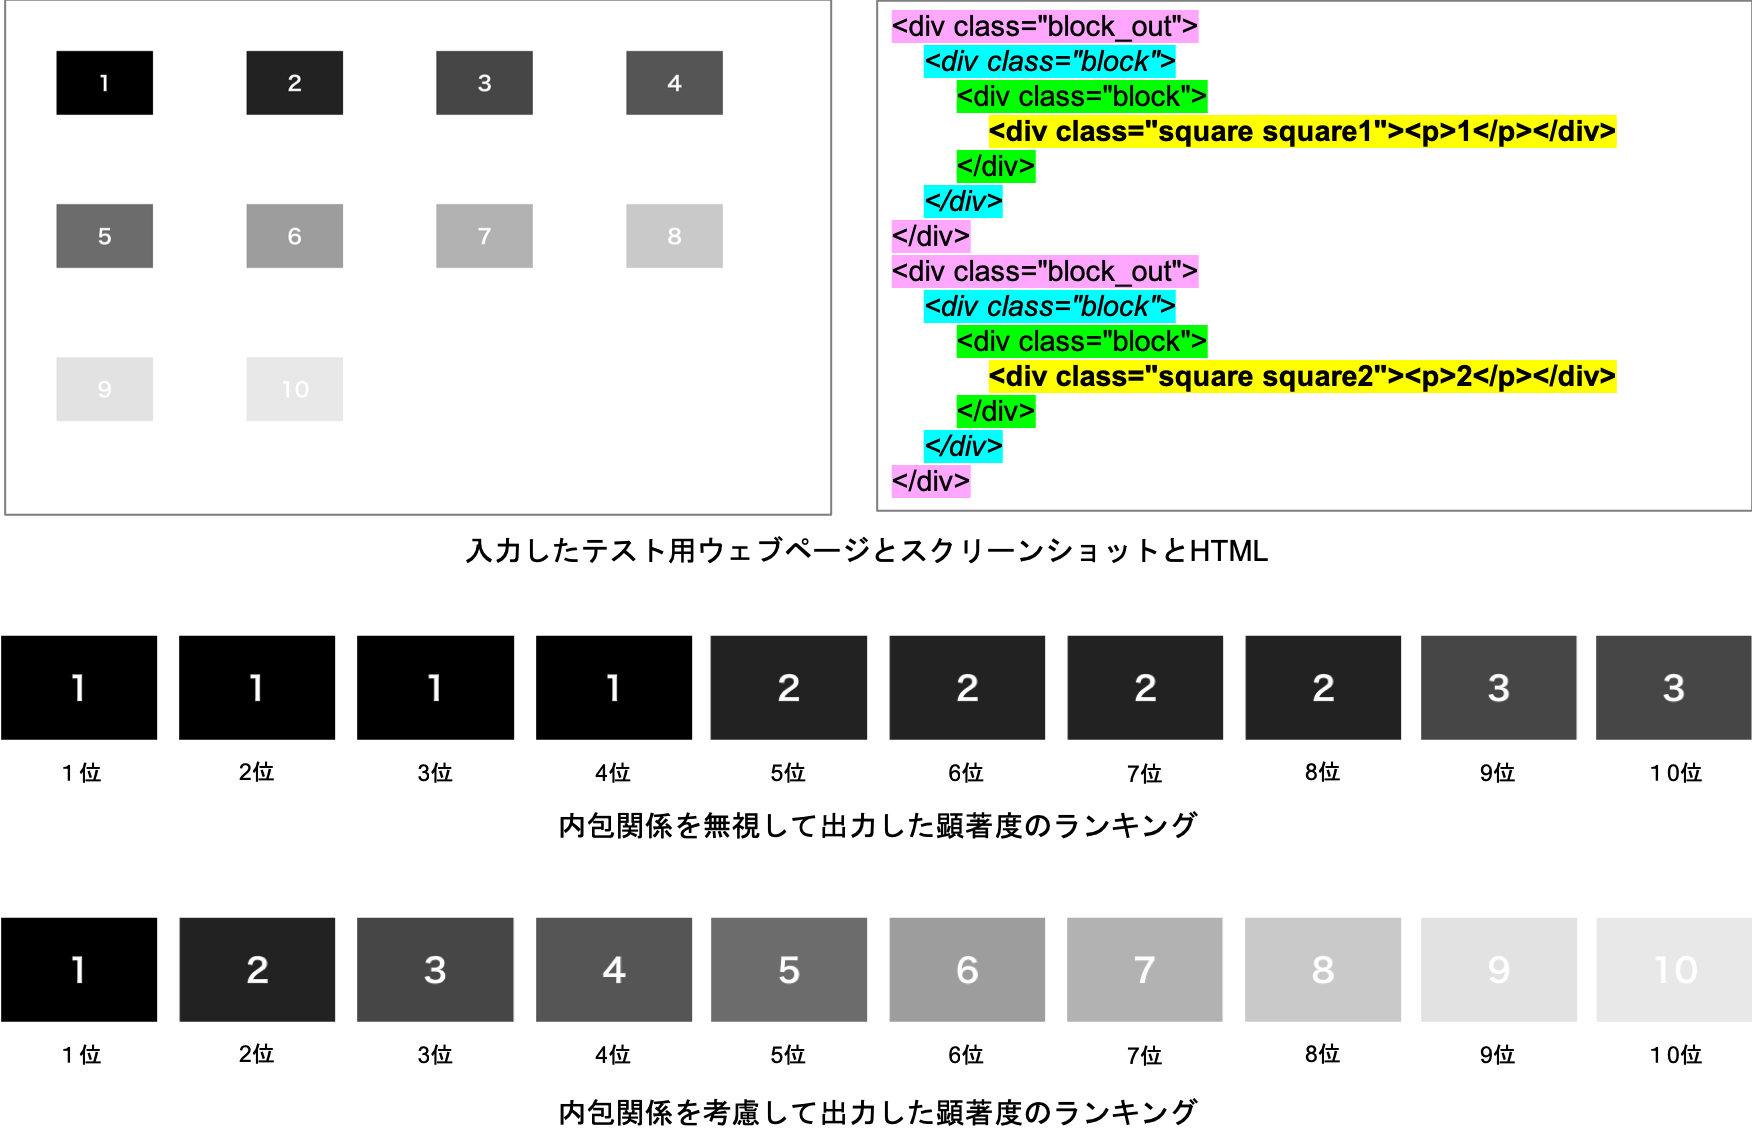
\includegraphics[width=12cm]{figures/06_rank.png}
    \caption{要素の内包関係を考慮した時としない時の顕著度ランキング}
    \label{fig_system4-rank}
\end{figure}

\subsubsection{顕著領域マップの生成}\label{subsec:system04-1}
\par 顕著領域マップの生成方法について説明する。第\ref{subsec:system03}節で計算した各要素の顕著度は上限なしの単精度浮動小数点型で表されている。要素を顕著度に応じた明度で塗りつぶす為にはコンピューター上で表現できる色の濃度の0$\sim$255の範囲内で表現する必要がある。本システムでは最も顕著度の高い要素の明度が$255$になるように顕著そを圧縮して、位置情報を取得した画面上に表示されている全ての要素の領域をこの顕著度を明度とした長方形で塗り潰す。

\par さらに、特に顕著度が高い重要領域を視覚化する為に第\ref{subsec:system04-1}項で作成した顕著度ランキングの指定個数(デフォルトは10個)の要素の外枠を顕著度が高い順に明るい緑色の線で描写する。このことにより、要素の塗りつ潰された明度の微妙な差異を簡単に見分ける事が可能になる。以上の作業を行う事で顕著領域マップの生成を行う。図\ref{fig_output-example}にテスト用ウェブページのURLを入力して生成された顕著領域マップの例を示す。なお、テストページには左図のように大きさが同じ長方形でそれぞれ異なる明度で塗りつぶされた要素が等間隔に並べられたページを作成して使用した。

\subsubsection{集約図の生成}\label{subsec:system04-2}
\par 集約図の生成方法について説明する。第\ref{subsec:system04-1}項で作成した顕著度ランキングを元に顕著度が特に高い指定個数(デフォルトは10個)の要素の領域をスクリーンショットから切り取りタイル状に並べる。本システムでは上段に上位2個を、中段に3位$\sim$5位の3個を、下段には6位$\sim$10位の5個を並べる事で顕著度が高い要素が大きい面積で表示されるようにした。図\ref{fig_output-example}に顕著領域マップの説明と同様のテスト用ウェブページのURLを入力して生成された集約図の例を示す。顕著度が高く目立ちやすい1番の要素から順番にタイル状に並べられてどの要素が注目されやすいのかを一目で確認する事が可能である。

\begin{figure}[H]
  \centering
  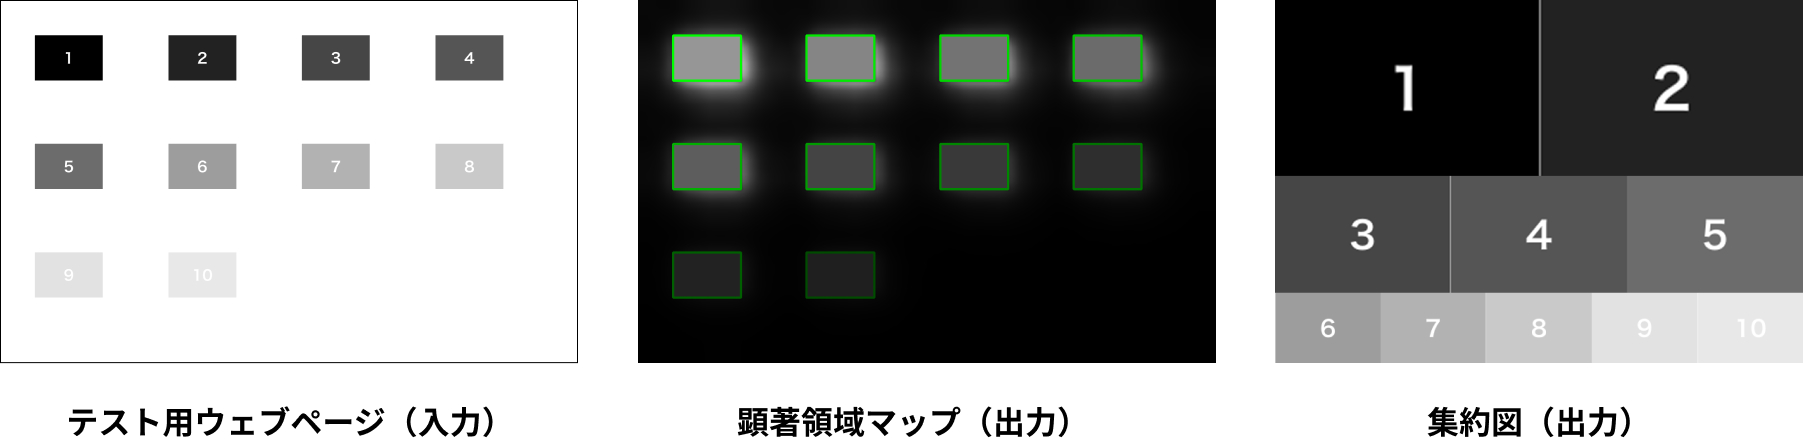
\includegraphics[width=12.5cm]{figures/06_example-output.png}
  \caption{生成される顕著領域マップと集約図の例}
  \label{fig_output-example}
\end{figure}
